% !TEX encoding = UTF-8
% !TEX program = lualatex

\documentclass[a4paper]{article}

\usepackage[left=1.5cm, right=1.5cm, top=1cm, bottom=2cm]{geometry}

\usepackage{mathtools, amssymb}
    \def\FF{\mathbf F}
    \def\tr{\operatorname{tr}}
    \def\BEC{\operatorname{BEC}}
    \def\BSC{\operatorname{BSC}}
    \def\AWGN{\operatorname{AWGN}}
    \def\bra#1{{\langle{#1}|}}
    \def\ket#1{{|{#1}\rangle}}

\usepackage{fontspec}
    \setmainfont{Noto Serif}
    \setsansfont{Noto Sans TC}
    \setmonofont{Noto Sans Mono}

\usepackage{tikz}

\begin{document}

\parindent 0pt
\parskip 1em

\newcounter{p}
\def\anssheet{}
\def\Problem#1{\stepcounter{p}[\thep]\addblank{#1}}
\def\addblank#1{\xdef\anssheet{\anssheet[\thep]\hbox to#1{}\hskip0pt plus#1}}

\newcounter{c}
\def\choice#1{%
    \stepcounter{c}\ifnum\value{c}=27\setcounter{c}{1}\fi%
    #1(\Alph{c})\nobreak\ 
}
\def\no{\choice{}}
\def\yes{\choice{}}

\section*{Error Correcting Codes - Final Mock}

\sffamily

考試時間 Test time 09:30:00 am to 12:00:00 pm; 2.5 hours.
以投影機時鐘為準 Using the projected clock.
在答案卷作答 Answer on answer sheet.
每個題號一分 One point per problem.
全對才給分 No partial credit.
可以帶紙製品 Materials made of paper are allowed.
聽音樂請帶耳機 Use earphones for music.
禁止操作電子設備 Do not touch electronic devices.
舉手問問題 Raise your hand to ask questions.

\rmfamily

$\FF_{4}$ is generated by 111 (i.e., $x^2 + x + 1$). \\
Its Zech table (i.e., $1 + \alpha^j = \alpha^{z(j)}$) is
0, 2, 1, 0.

$\FF_{8}$ is generated by 1011 (i.e., $x^3 + x + 1$). \\
Its Zech table (i.e., $1 + \alpha^j = \alpha^{z(j)}$) is
0, 3, 6, 1, 5, 4, 2, 0.

$\FF_{16}$ is generated by 10011 \\
(i.e., $x^4 + x + 1$).
Its Zech table is \\
0, 4, 8, 14, 1, 10, 13, 9, 2, 7, \\
5, 12, 11, 6, 3, 0.

$\FF_{64}$ is generated by 1011011 \\
(i.e., $x^6 + x^4 + x^3 + x + 1$).
Its Zech table is \\
0, 56, 49, 13, 35, 30, 26, 8, 7, 27, \\
60, 23, 52, 3, 16, 34, 14, 39, 54, 48, \\
57, 42, 46, 11, 41, 58, 6, 9, 32, 44, \\
5, 59, 28, 38, 15, 4, 45, 43, 33, 17, \\
51, 24, 21, 37, 29, 36, 22, 61, 19, 2, \\
53, 40, 12, 50, 18, 62, 1, 20, 25, 31, \\
10, 47, 55, 0.

$\FF_{128}$ is generated by 10000011 \\
(i.e., $x^7 + x + 1$).
Its Zech table is \\
0, 7, 14, 63, 28, 54, 126, 1, 56, 90, \\
108, 87, 125, 55, 2, 31, 112, 43, 53, 29, \\
89, 57, 47, 82, 123, 105, 110, 66, 4, 19, \\
62, 15, 97, 77, 86, 109, 106, 46, 58, 100, \\
51, 75, 114, 17, 94, 68, 37, 22, 119, 122, \\
83, 40, 93, 18, 5, 13, 8, 21, 38, 104, \\
124, 88, 30, 3, 67, 95, 27, 64, 45, 107, \\
91, 79, 85, 78, 92, 41, 116, 33, 73, 71, \\
102, 118, 23, 50, 101, 72, 34, 11, 61, 20, \\
9, 70, 74, 52, 44, 65, 111, 32, 117, 103, \\
39, 84, 80, 99, 59, 25, 36, 69, 10, 35, \\
26, 96, 16, 115, 42, 113, 76, 98, 81, 48, \\
121, 120, 49, 24, 60, 12, 6, 0.

\vskip-15cm
\leftskip10.5cm

$\FF_{32}$ is generated by 100101 \\
(i.e., $x^5 + x^2 + 1$).
Its Zech table is \\
0, 18, 5, 29, 10, 2, 27, 22, 20, 16, \\
4, 19, 23, 14, 13, 24, 9, 30, 1, 11, \\
8, 25, 7, 12, 15, 21, 28, 6, 26, 3, \\
17, 0.

$\FF_{256}$ is generated by 100011101 \\
(i.e., $x^8 + x^4 + x^3 + x^2 + 1$).
Its Zech table is \\
0, 25, 50, 223, 100, 138, 191, 112, 200, 120, \\
21, 245, 127, 99, 224, 33, 145, 68, 240, 92, \\
42, 10, 235, 196, 254, 1, 198, 104, 193, 181, \\
66, 45, 35, 15, 136, 32, 225, 179, 184, 106, \\
84, 157, 20, 121, 215, 31, 137, 101, 253, 197, \\
2, 238, 141, 147, 208, 63, 131, 83, 107, 82, \\
132, 186, 90, 55, 70, 162, 30, 216, 17, 130, \\
64, 109, 195, 236, 103, 199, 113, 228, 212, 174, \\
168, 160, 59, 57, 40, 170, 242, 167, 175, 203, \\
62, 209, 19, 158, 202, 176, 251, 190, 139, 13, \\
4, 47, 221, 74, 27, 248, 39, 58, 161, 71, \\
126, 246, 7, 76, 166, 243, 214, 122, 164, 153, \\
9, 43, 117, 183, 180, 194, 110, 12, 140, 239, \\
69, 56, 60, 250, 177, 144, 34, 46, 5, 98, \\
128, 52, 218, 150, 135, 16, 217, 53, 206, 188, \\
143, 178, 226, 119, 201, 159, 169, 41, 93, 155, \\
81, 108, 65, 182, 118, 227, 114, 87, 80, 156, \\
85, 211, 229, 232, 79, 88, 95, 134, 151, 37, \\
124, 29, 163, 123, 38, 249, 61, 204, 149, 219, \\
97, 6, 247, 28, 125, 72, 23, 49, 26, 75, \\
8, 154, 94, 89, 187, 207, 148, 205, 54, 91, \\
241, 171, 78, 233, 116, 44, 67, 146, 142, 189, \\
252, 102, 237, 3, 14, 36, 152, 165, 77, 172, \\
231, 230, 173, 213, 244, 22, 73, 222, 51, 129, \\
18, 210, 86, 115, 234, 11, 111, 192, 105, 185, \\
133, 96, 220, 48, 24, 0.

\leftskip0cm

\vskip-1.5cm

\[\begin{tikzpicture} [overlay, rotate=90, yshift=0.5cm]
    \draw (0, 0) -- (10, 0);
    \foreach \x in {0, ..., 9} {
        \pgfmathtruncatemacro\xa{floor(\x / 10)}
        \pgfmathtruncatemacro\xb{mod(\x, 10)}
        \draw (\x, 0) -- +(0, 0.3) node [left] {$\xa.\xb$};
        \draw (\x.5, 0) -- +(0, 0.2);
        \foreach \y in {1, ..., 9} {
            \draw (\x + \y/10, 0) -- +(0, 0.1);
        }
    }
     \foreach \k in {1, ..., 9} {
        \draw ({10 * log10(\k)}, 0) -- +(0, -0.3)
            node [right] {$\log_{10}\k$};
        \draw ({10 * log10(\k + 0.5)}, 0) -- +(0, -0.2);
        \foreach \l in {1, 2, 3, 4, 6, 7, 8, 9} {
            \draw ({10 * log10(\k + 0.\l)}, 0) -- +(0, -0.1);
        }
    }
\end{tikzpicture}\]

For questions with precision requirements,
(2x) means that your answer should be in $[a/2, 2a]$,
(5x) means  $[a/5, 5a]$.
For this kind of questions, answer in scientific notation such as 1.2e345.

\Problem{2em}
Parallel combination makes channels
\yes less noisy
\no more noisy

\Problem{2em}
Serial combination makes channels
\no less noisy
\yes more noisy

\Problem{2em}
Parallel combination turns two BECs into
\yes a BEC for sure
\no a generic channel.
PS.\ For this type of problem where one choice implies the other,
you must chose the strongest choice.
That is, running a red light will be fined $\ge 1800$,
not $\ge 1$.

\Problem{2em}
Serial combination turns two BECs into
\no a BEC for sure
\yes a generic channel

\Problem{2em}
Parallel combination turns two BSCs into
\no a BSC for sure
\yes a generic channel

\Problem{2em}
Serial combination turns two BSCs into
\yes a BSC for sure
\no a generic channel

\Problem{2em}
A bounded martingale $M_n \in [0, 1]$ converges to
\no a random variable $M_\infty \in \{0, 1\}$ for sure
\yes a random variable $M_\infty \in [0, 1]$
\no unfortunately it may not converge

\Problem{2em}
A submartingale is like a martingale,
except that tomorrow's expectation can be better than today's.
A bounded submartingale $S_n \in [0, 1]$ converges to
\no a random variable $S_\infty \in \{0, 1\}$ for sure
\yes a random variable $S_\infty \in [0, 1]$
\no unfortunately it may not converge

\Problem{2em}
If a submartingale $Z_n$ converges to $Z_\infty \in \{0, 1\}$,
then the probability $P(Z_\infty = 1)$ is
\yes $\ge Z_0$
\no $\le Z_0$
\no not necessarily comparable to $Z_0$.

\Problem{2em}
Using the Zech representation,
what is $12 + 34$ in $\FF_{64}$?

\Problem{2em}
Using the Zech representation,
what is $56 + 78 + 90$ in $\FF_{256}$?

\Problem{2em}
With the polynomial representation
(notice how binary strings correspond to polynomials in the table above),
what is $11011 \cdot 10101$ in $\FF_{32}$?

\Problem{2em}
With the polynomial representation
(notice how binary strings correspond to polynomials in the table above),
what is $0001111 \cdot 1110000 \cdot 0011100$ in $\FF_{128}$?

\Problem{2em}
A tetrahedral erasure channel
TEC$(p, q, r, s, t)$ is a channel with input alphabet $\FF_4$
and output alphabet $\{0, 1, \ast\}^3$.
Note that there is a trace function $\tr\colon \FF_4 \to \FF_2$
that is the same trace function as if $\FF_4$
is represented as 2-by-2 matrices over $\FF_2$.
Given an input $x \in \FF_4$, the TEC outputs
\begin{itemize}
    \item $(\tr(x\omega), \tr(x), \tr(x/\omega))$ w.p.\ $p$,
    \item $(\tr(x\omega), \ast, \ast)$ w.p.\ $q$,
    \item $(\ast, \tr(x), \ast)$ w.p.\ $r$,
    \item $(\ast, \ast, \tr(x/\omega))$ w.p.\ $s$, and
    \item $(\ast, \ast, \ast)$ w.p.\ $t$.
\end{itemize}
Here, $\omega \in \FF_4$ is a fixed element that is not in $\FF_2$.
Show that, if I send $a \in \FF_2$ through BEC$(\phi)$
and $b \in \FF_2$ through BEC$(\psi)$,
then this is equivalent to sending $a + b\omega$ through a TEC.
Express the pqrst of this TEC using $\phi$ and $\psi$.

\Problem{2em}
Find the conditional entropy of TEC$(p, q, r, s, t)$.

\Problem{2em}
Length-$2$ quaternary polar code is used over TEC.
Show that the parallel combination of
TEC$(p, q, r, s, t)$ and TEC$(p', q', r', s', t')$ is a TEC
by finding the new pqrst using $p, \dotsc, t'$

\Problem{2em}
The same problem for serial combination.

\Problem{2em}
Recall that parallel and serial combinations
turn the $x$ in BEC$(x)$ to $x \pm x (1 - x)$.
So the the difference between the conditional entropies
of the parallel and serial combinations is $2 x (1 - x)$.
Now, for the special case TEC$(p, r, r, r, t)$,
express (simplify) the difference between the conditional entropies
of the parallel and serial combinations.

\Problem{2em}
Alice is sending some bits.
The channel Bob sees is BEC with erasure probability $0.1$.
The channel Eve sees is BEC with capacity $0.1$.
Find a sequence of P (parallel) and S (serial)
so that Bob's new erasure probability is less than $0.01$,
and Eve's new capacity is less than $0.01$.
(If your answer is too pathological for my computer to double-check,
I will ask you to show me a proof of correctness.)

\Problem{2em}
Show that, for any $\varepsilon > 0$, there exists a $\delta > 0$ such that,
if $H(W) < \delta$ for some BMSC $W$, then $Z(W) < \varepsilon$.
Here, $H$ is the conditional entropy (equivocation),
and $Z$ is the Bhattacharyya parameter of $W$.

\Problem{2em}
Show that, for any $\varepsilon > 0$, there exists a $\delta > 0$ such that,
if $Z(W) < \delta$ for some BMSC $W$, then $H(W) < \varepsilon$.

\Problem{2em}
Prove that, for any $\varepsilon > 0$, there exists a $\delta > 0$ such that,
if $H(W) > 1 - \delta$ for some BMSC $W$, then $Z(W) > 1 - \varepsilon$.

\Problem{2em}
Prove that, for any $\varepsilon > 0$, there exists a $\delta > 0$ such that,
if $Z(W) > 1 - \delta$ for some BMSC $W$, then $H(W) > 1 - \varepsilon$.

\Problem{2em}
Let $W$ and $V$ be two BMSCs.
If there exists a randomized function $f$ such that the output of $W$
can be simulated by passing the output of $V$ through $f$, we say that
$W$ is a \emph{degrade} of $V$, and $V$ is an \emph{upgrade} of $W$.
For any $0 < p < q < 1$, it is known that BEC$(q)$ is a degrade of BEC$(p)$.
What does the randomized function $f$ look like?

\Problem{2em}
For any $0 < p < q < 1$, it is known that BSC$(q)$ is a degrade of BSC$(p)$.
What does the randomized function $f$ look like?

\Problem{2em}
For any $0 <  < s < 1$, it is known that AWGN$(s)$ is a degrade of
AWGN$(t)$, where $s$ and $t$ are variances, and the inputs are $\pm1$.
What does the randomized function $f$ look like?

\Problem{2em}
Show that, if $W$ is a degrade of $V$,
then $W \star U$ is a degrade of $V \star U$,
where $\star$ means parallel combination.

\Problem{2em}
Do the same problem if $\star$ means serial combination.

\Problem{2em}
Suppose that the channel Bob sees is BEC$(p)$,
and the channel Eve sees is BEC$(q)$.
Suppose that Eve's channel must output erasure if Bob's channel does.
So Eve's channel is a \emph{physical} degrade of Bob's,
not just a \emph{statistical} degrade.
Now, for any sequence $\sigma \in \{p, s\}^n$ of parallel and serial,
show that BEC$(q)^\sigma$ is a physical degrade of BEC$(p)^\sigma$.

\Problem{2em}
Let us analyze $(3, 6)$-LDPC using density evolution.
When the underlying channel is BEC$(1/3)$,
how many iterations of belief propagation do you need
to bring the fraction of erased VNs to $1/10$ or below.

\Problem{2em}
When the underlying channel is $W$,
the LLRs on each VN is a random variable.
The distribution of these random variable changes after one iteration of BP.
Which channel's LLR has the same distribution as that?

\Problem{2em}
Which channel describes the distribution of LLRs after two iterations of BP?

\Problem{2em}
Polar codes have a great ability called \emph{rate matching}.
At length $2^n$, polar codes offer codes of rates
$1/2^n, 2/2^n, \dotsc, (2^n - 1) / 2^n$
by selecting info sets and frozen sets of proper sizes.
That is, one chip can handle multiple code rates by reusing decoder area.
To determine info and frozen sets, the following procedure is used:
Assume that every channel is a frozen bit, that is,
the decoder always has the correct ``$u_1$'' when decoding for ``$u_2$''.
However, we still record if a $u_i$ is mis-decoded.
Now, for a polar code of length $4$,
suppose that only the second BEC outputs erasure,
which bit-channel(s) is mis-decoded?
%
PS.\ For those of you who does not think BEC is a good model of channel,
imagine that the same question is asked for BSC.

\Problem{2em}
The same question but the first and the last BEC output erasures.

\Problem{2em}
In the bit-flip basis, also called the Z-basis,
$\bra\uparrow$ is the row vector $[1\, 0]$ and
$\bra\downarrow$ is the row vector $[0\, 1]$.
In the phase basis, also called the X-basis,
$\bra+$ is the row vector $[1\, 1]/\sqrt2$, and
$\bra-$ is the column vector $[1\, -1]/\sqrt2$.
Find the 2-by-2 matrix $H$ such that
$\bra\uparrow H = \bra+$ and $\bra\downarrow H = \bra-$.

\Problem{2em}
Find the matrix $H'$ that does the opposite direction of change of basis.
That is, $\bra+ H' = \bra\uparrow$ and $\bra- H' = \bra\downarrow$.

\Problem{2em}
The NOT gate in the phase basis maps
\begin{itemize}
    \item $\bra+$ to $\bra-$, and
    \item $\bra-$ to $\bra+$.
\end{itemize}
Express this NOT gate in the bit flip basis.

\Problem{2em}
The CNOT gate in the phase basis maps
\begin{itemize}
    \item $\bra{++}$ to $\bra{++}$,
    \item $\bra{+-}$ to $\bra{+-}$,
    \item $\bra{-+}$ to $\bra{--}$, and
    \item $\bra{--}$ to $\bra{-+}$.
\end{itemize}
Express this CNOT gate in the bit flip basis.

\Problem{2em}
Find a 2-by-2 matrix $S$ such that $S^2$
is the NOT gate in the bit flip basis.

\Problem{2em}
PS is
\tikz [baseline=-0.5ex] \draw
    (0, 0) circle (0.05)
    (0, 0) to [bend left] (1, 0.5) circle (0.05)
    (0, 0) to [bend right] (1, -0.5) circle (0.05)
    (1, 0.5) to [bend left] (2, 0) circle (0.05)
    (1, -0.5) to [bend right] (2, 0)
;
Draw PPSPS.

\Problem{2em} (2x)
Express $\binom{1000}{333}$ in scientific notation.

\Problem{2em} (2x)
Express $Z(\mathrm{BSC}(0.1)^{ppppp})$ in scientific notation.

\Problem{2em} (2x)
Express $Z(\mathrm{BSC}(0.1)^{sssss})$ in scientific notation.

\Problem{2em} (2x)
Define $T(\BSC(p))$ as $|1 - 2p|$.
Define the $T$ of any convex combination of BSCs to be
the same convex combination of the $T$'s of the BSCs.
Express $T(\BSC(0.2345)^p)$ in scientific notation.

\Problem{2em} (2x)
Express $T(\AWGN(0.2345))$ in scientific notation.

\Problem{2em}
\Problem{2em}
\Problem{2em}
\Problem{2em}
\Problem{2em} (5x)
There will be five problems that ask you to guess
certain quantities regarding real-world usage of error-correcting codes.

\clearpage

\cleardoublepage

\section*{Error Correcting Codes - Final Mock}

\parskip0pt
\advance\lineskip1cm plus1fil
\advance\baselineskip1cm plus1fil

Name (zh or en) \hfil Student ID

\anssheet

\end{document}